% A Three fold Brochure based on the Latex document class-leaflet
 
\documentclass[notumble,10pt,a4paper]{leaflet} 

% notumble - By default (tumble) the contents of the backside sheet is printed upside down. The option no tumble supresses that.

% Please find the remaining options at http://ctan.math.illinois.edu/macros/latex/contrib/leaflet/leaflet-manual.pdf
\usepackage[utf8x]{inputenc}
\usepackage{fontspec}

\usepackage{color}
\usepackage{flowfram}
\usepackage{graphicx}
\usepackage{wrapfig}
\usepackage{hyperref}      % For including urls
\usepackage{rotating}
\usepackage{multirow}
\usepackage{array}
\usepackage{multirow}
\usepackage{titlesec}
\usepackage[usenames,dvipsnames]{xcolor}
\usepackage{setspace}    % Adjust line spacing    
\onehalfspacing          % Adjust line spacing  \doublespacing 
\usepackage[inline]{enumitem}
%\titleformat*{\subsection}{\color{Blue}}

%FONT Change
%\renewcommand{\familydefault}{cmss} 
%To Draw a horizontal Line
\newcommand{\sectionline}{
  \nointerlineskip \vspace{\baselineskip}
  \hspace{\fill}\rule{0.8\linewidth}{.7pt}\hspace{\fill}
  \par\nointerlineskip \vspace{\baselineskip}
}
%\AddToBackground{2}{\includegraphics[width=29.7cm]{bkf}}
%\AddToBackground{2}{\includegraphics[width=29.7cm]{cmy}}

% To create a border along the top of each page
% To change border color just search on internet for cmyk colour codes and change the values in the brackets after the option cmyk

\vtwotonetop{1cm}{0.6\paperwidth}{[cmyk]{0.35,0,0.67,0.41}}{topleft}%
{0.4\paperwidth}{[cmyk]{0.35,0,0.67,0.41}}{topright}

% To create a border along the bottom of each page
% To change border color just search on internet for cmyk colour codes and change the values in the brackets after the option cmyk

\vtwotonebottom{1cm}{0.6\paperwidth}{[cmyk]{0.35,0,0.67,0.41}}{bottomleft}%
{0.4\paperwidth}{[cmyk]{0.35,0,0.67,0.41}}{bottomright}


\usepackage{listings}
\usepackage{xcolor}
\definecolor{codegreen}{rgb}{0,0.6,0}
\definecolor{codegray}{rgb}{0.5,0.5,0.5}
\definecolor{codepurple}{rgb}{0.58,0,0.82}
\definecolor{backcolour}{rgb}{0.95,0.95,0.92}

\lstdefinestyle{mystyle}{
    backgroundcolor=\color{backcolour},   
    commentstyle=\color{codegreen},
    keywordstyle=\color{magenta},
    numberstyle=\tiny\color{codegray},
    stringstyle=\color{codepurple},
    basicstyle=\ttfamily\footnotesize,
    breakatwhitespace=false,         
    breaklines=true,                 
    captionpos=b,                    
    keepspaces=true,                 
    numbers=none,                    
    numbersep=5pt,                  
    showspaces=false,                
    showstringspaces=false,
    showtabs=false,                  
    tabsize=2
}

\lstset{style=mystyle}


\begin{document}
\begin{center}
	{\Large Arduinio} \\[.3cm]
	%\textit{on}\\[.4cm]
	{\huge {Cheat Sheet}}\\ [.3cm]
	
	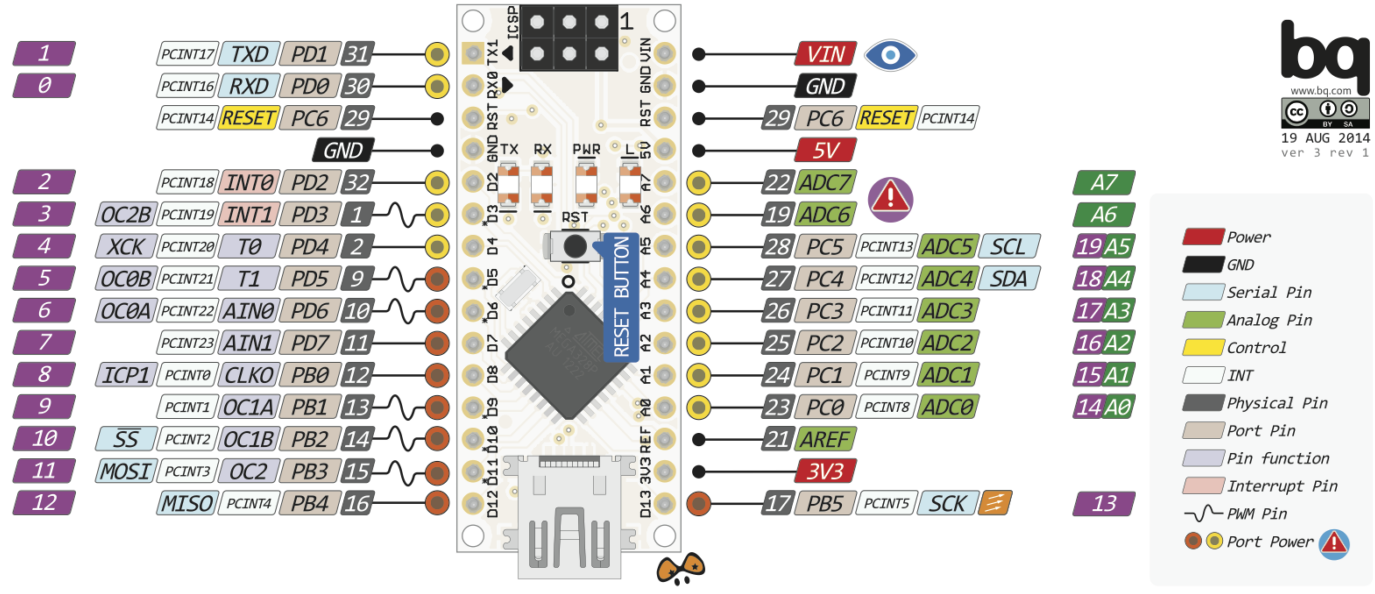
\includegraphics[width=\linewidth]{pictures/nanoFull.png}\\
	\label{fig:Pinout}

	
	\vfill
	created by\\ 
	\textbf{WAK-Lab e.V. Eisenach}\\
	Web:\url{https://wak-lab.org}
\end{center}


\thispagestyle{empty} 
\newpage
\subsection{\large{Arduino IDE}}
Die Arduino IDE ist das Programm, mit dem du Microcomputer, wie etwa den Arduino relativ einfach programmieren kannst. Wenn du später fortgeschrittener bist, kannst du auch andere Programme, wie etwa Visual Studio Code verwenden. Dateien für den Arduino werden mit der Dateiendung ".ino" gespeichert und sind in der Sprache C++ geschrieben.\\
\subsection{\large{Programmstruktur}}
Das Programm besteht im wesentlichen aus einer \textit{"setup()"} Funktion, die beim Programmstart aufgerufen wird und eine \textit{"loop()"} Funktion, die sich automatisch immer wieder wiederholt. Im deutschen nennt man diese Art der Funktion "Schleife".\\
Damit sich der Computer Dinge merken kann, nutzen wir sogenannte Variablen.
Diese haben verschiedene Typen, doch das ist ganz einfach:
\begin{lstlisting}[language=c, caption=Datentypen in C]
int eineZahl = 27; // "int" für ganze Zahlen (von -32768 bis 32767)
string einWort = "Hallo:)"; // "string" für Wörter oder Sätze
double eineKommazahl = 5.2; // "double" für Zahlen mit Komma
boolean wahr = true; // "boolean" für Wahr oder Falsch
boolean falsch = false;
void // "void" für nichts (wird bei Funktionen genutzt, die nichts zurückgeben sollen)
// "//" für Kommentare

\end{lstlisting}
\hfill \break \hfill \break \hfill \break
Damit der Computer etwas berechnen kann, brauchen wir Funktionen. Neben den Standard-Funktion  \textit{"setup()"} und \textit{"loop()"} können wir uns auch eigene bauen. Der Vorteil davon ist, dass man damit recht unkompliziert lange Rechnungen wiederholen kann, ohne den kompletten Code neu schreiben zu müssen.
Das ganze geht so:

\begin{lstlisting}[language=c, caption=Funktionen in C]
Datentyp Name (Datentyp Parameter) {
	//Parameter dienen der Weiterverwendung von Variablen aus dem Hauptprogramm
	Code der Funktion; 
	return Variable; //Variable muss den gleichen Datentyp haben, wie der zuvor vor dem Funktionsnamen definierte Datentyp
	//in void-Funktionen brauchen wir kein "return"
}
//Ein Beispiel für eine eigene Funktion:
int plusEins (int zahl) {
	return zahl + 1; //addiere eins zu der Zahl und gebe sie zurück
}
//So sehen die Standard-Funktionen aus, bevor du sie anpasst:
void setup() {
  // Dieser Code wird beim Start aufgerufen
  // Diese Variable existiert nur so Lange Setup läuft
  int EineLokaleVariable;  
}

void loop() {
  // Dieser Code wird immer wieder aufgerufen
  // Diese Variable existiert dauerhaft und behält ihren Wert beginnend mit 0
  int eineLokaleVariable = 0; 
  int eineLokaleVariablePlusEins = plusEins(eineLokaleVariable);
}
\end{lstlisting}
\subsection{\large{Bibliotheken verwenden}}
Bibliotheken sind Voreinstellung und Bauanleitungen für Funktionalitäten die wir einfach benutzen wollen ohne uns groß in Details zu verstricken. Die wichtigsten Bibliotheken sind bereits automatisch eingebunden ohne dass wir davon etwas in der Arduino IDE mitbekommen.
\subsection{Serial}
Die Verbindung zum "seriellen Monitor" ermöglicht uns, dass der Mikrocomputer Texte und Zahlen an uns senden kann. Damit können wir lesen, was der Prozessor (Rechner) gerade macht. 
\begin{lstlisting}[language=c, caption=Ausgabe von Text an den Programmierer]
void setup() {
  Serial.begin(9600); //diesen Command im Setup benötigen wir, damit der Computer weiß, wie er mit uns reden soll
}

void loop() { //Diese Funktion schreibt uns jede Sekunde "Hallo Welt"
  Serial.println("Hallo Welt");
  // Eine Wartezeit von 1000 Millisekunden wartet 1 Sekunde    
  delay(1000);        
}
\end{lstlisting}
\newpage
\subsection{\large{Eingänge}}
Damit wir z.B. Knöpfe oder Sensoren verwenden können, müssen wir dem Computer sagen, an welchem Pin wir unsere Sachen angeschlossen haben. Welcher Pin was kann am Mikrocontroller steht im Datenblatt von diesem. Rechts findest du das Datenblatt vom "Arduino Nano".
\begin{lstlisting}[language=c, caption=Eingänge am Arduino lesen]
void setup() {
   // Pin 2 als Eingang definieren
  pinMode(2, INPUT); 
}
void loop() {
  // Digitaler Eingang 2 einlesen
  int knopfStatus = digitalRead(2); // digital gibt uns an/aus an
  // Analogen Eingang A0 einlesen
  int sensorWert = analogRead(A0); //analog gibt uns genaue Spannungswerte am jeweiligen Pin an
}
\end{lstlisting}
\hfill \break \hfill \break \hfill \break \hfill \break \hfill \break \hfill \break \hfill \break \hfill \break \hfill \break \hfill \break \hfill \break \hfill \break \hfill \break \hfill \break
\subsection{\large{Ausgänge}}
Für Ausgänge machen wir genau das gleiche, nur mit anderen Funktionsaufrufen:
\begin{lstlisting}[language=c, caption=Ausgänge am Arduino nutzen]
void setup() {
   // Pin 2 als Ausgang definieren
  pinMode(2, OUTPUT); 
  pinMode(A0, OUTPUT);
}
void loop() {
  digitalWrite(2, HIGH); //setzt die Spannung am Pin 2 auf den Maximalwert
  analogWrite(3, 120); //setzt die Spannung am Pin 3 auf 120 den Wert 120 (Maximal gehen 255)
  //mit analogWrite kann man z.B. die Helligkeit einer LED variabel einstellen, wenn die LED das erlaubt
  delay(1000);
}
\end{lstlisting}




Text

\begin{itemize*} %use itemize without the asterik to get the usual list appearance
	\item Test
\end{itemize*}

\subsection{\large{Section 2}}
\noindent
\begin{tabular}{@{}ll}
	Tabelle & Datum\\
	Eintrag    & Info\\
\end{tabular}

{\large\textbf{{Contact}}}\\
\url{info@wak-lab.org}

\begin{center}
\textbf{Apply} \\
Hier könnte ihr QR-Code stehen\\
%\begin{figure}[h!]
%	\centering
%	\includegraphics[width=0.3\linewidth]{QR-Code}
%\end{figure}
\end{center}

\newpage

\section{\large{Section 3}}


\subsection{\large{Contact}}
WAK-Lab.e.v\\
CNebestraße 24\\
99817 Eisenach\\
Germany\\
Email:  \url{info@wak-lab.org}

\newpage
\vspace*{\fill}
\begin{center}
%	\begin{figure}[h!]
%		\centering
%		\includegraphics[width=0.3\linewidth]{Kontakt bild}
%	\end{figure}
%	\Large{\textbf{\url{https://wak-lab.org}}}	
\end{center}
\vspace*{\fill}


\end{document}
